本章会介绍API描述性知识抽取系统的设计与具体实现,以及根据API描述性知识图谱设计的API描述性知识汇总应用的设计与实现。本文实现的API描述性知识抽取系统分为三个模块,分别是语料库生成模块、抽取主题模块以及知识图谱构建模块。在下文中,将会对这三个模块以及汇总应用的设计与具体实现一一进行介绍。

\section{语料库生成模块}
语料库生成模块可以细分为三个子模块,分别是从数据库中获取Stack Overflow帖子的帖子获取模块,对帖子中的文本进行处理的帖子预处理模块,以及最后的fastText文本分类器模块。

\subsection{帖子获取模块}如前文章节3.4.1中介绍的,本文提出的API描述性知识抽取方法的抽取对象来自软件开发问答网站Stack Overflow。Stack Overflow网站会定期将论坛中的所有数据导出成SQL备份文件并公开发布,运行该备份文件可以将Stack Overflow中所有的帖子导入到本地SQL数据库中。Stack Overflow帖子数据中包括了帖子的标题、正文、标签列表、帖子得分、帖子类型等属性。本文设计了一个工具类DatabaseManager,使用pymysql库来实现本系统与SQL数据库的连接,根据前文章节3.2.1中设计的筛选条件,本方法使用SQL查询语句来完成数据库帖子的过滤与获取。由于在帖子数据中,只有问题类型的帖子才有标签列表这一属性,所以需要通过回答类型帖子拥有的“归属问题ID”字段来定位一个回答帖子属于哪个问题帖子,再通过查询原问题帖子的标签列表来进行筛选。使用sql语句“SELECT * FROM stackoverflow\_2021.posts AS t1 JOIN stackoverflow\_2021.posts AS t2 ON t1.parentId = t2.ID WHERE t2.tags LIKE '\%java\%' AND t1.posttypeid = 2 AND t1.score\textgreater{0};”可以检索到符合上述要求的帖子。得到需要的Stack Overflow帖子后,本模块以json的文件形式将其保存到本地,等待下一步的处理。

\subsection{帖子预处理模块}
本模块的主要功能是对帖子获取模块保存下来的Stack Overflow帖子进行处理。Stack Overflow帖子的正文是以HTML语言形式保存在数据库中的,为了得到本方法所需要的纯文本,还需要对其进行解析。Python库BeautifulSoup提供了解析HTML文本的方法,用户可以像操作一颗树一样对HTML文本进行遍历、修改。在帖子正文中,除了自然语言文本以外,还存在着API提及和大段的代码片段。通常来说,用户在编写帖子时会将大段的代码片段用标签<pre><code></code></pre>包裹起来,以保持代码的格式。而由于API提及通常只有一个词,所以有些用户会将其用<code></code>标签包裹起来,而有些用户则是直接将其插在自然语言文本中。故在这里本模块只将大段的代码片段用占位符$-CODE-$替换,将API提及的识别放到后面做。通过使用BeautiflSoup,本模块将HTML文本中的标签全部去除,并将其中的大段代码片段替换为占位符。

得到去除代码片段的纯文本后,帖子预处理模块会使用spaCy对它们进行自然语言解析。如前文介绍的,由于软件工程领域的文本特性,需要对分词工具Spacy进行自定义修改,以使分句结果满足要求。根据前文章节3.3.2所总结的影响分句的文本特殊情况,本文对spaCy的tokenizer模块进行分句规则的修改,tokenizer模块设定有分句的前缀规则、中缀规则、后缀规则和特殊规则。本文根据上述句子的特点,对中缀规则进行修改,使其不再将连接符号断句;对后缀规则进行修改,使其不再对API提及中的句号和圆括号、尖括号进行分句。

将文本完成分句后,本方法使用表3-1中设计的正则表达式对所有句子进行匹配,找到包含API提及的句子,并将句子中的API提及使用占位符$-API-$替换,最后将替换后的句子和句子中的API提及一起保存下来。

本模块设计了两个功能类,分别是SentenceManager类和NLPUtil类,其中SentenceManager类应用了BeautilfulSoup库和re库,用于完成HTML标签解析以及API提及识别替换功能。为了保证在调用spaCy库进行自然语言处理的时候重复使用同一个spaCy模型以节省内存空间,NLPUtil类以单例模式设计并封装了spaCy模型。在本方法第一次加载NLPUtil类时,会生成唯一一个spaCy模型对象,并对这个spaCy模型的tokenizer模块进行修改。在之后的抽取流程中只要调用NLPUtil类提供的接口函数就可以对自然语言文本进行分句、分词等操作。

在后续的抽取主体模块中,spaCy会被频繁地调用来解析一个API描述性知识句子。而在知识元组匹配和语言模式匹配的过程中,同一个句子会被spaCy多次重复解析,这造成了性能的浪费。为了优化本方法的流程执行效率,本方法对NLPUtil类添加了缓存功能,设计了一个NLPCache子类,每当一个句子被spaCy解析成doc对象,就将句子本身和doc对象作为键值对保存到Python字典中。在调用NLPUtil类解析一个句子时,首先检查这个句子是否已经存在于NLPCache中,如果存在则直接返回解析好的doc对象,如果不存在再调用spaCy模型进行解析。NLPCache还基于Python pickle模块实现了保存加载功能,能将解析好的doc对象以二进制文件的形式保存下来,这样在重复运行抽取主体模块时便能将之前已解析过的文本直接读取到内存中,加快了运行速度。

\subsection{fastText文本分类模块}
语料库生成的最后一个子模块是文本分类模块。本方法在这里训练了一个fastText文本分类器,用于在带有API提及的句子中找到API描述性知识句子。本方法从帖子预处理模块中处理得到的带有API提及的句子中随机采样得到2000条,并人工对其进行标注。为了保证标注数据的准确性,本文邀请了两位具有3年以上Java开发经验的研究生对这2000条句子进行标注,判断它们是否为API描述性知识句子。在进行标注前,我们还对两位标注者进行了培训,统一了API描述性知识句子的标注标准。当两位标注者的标注结果出现不一致时,会邀请第三位仲裁者,对这一条数据进行仲裁。

标注完成后,本文发现样本数据中正负样本的比例差距较大,在2000个句子之中,只有542个句子被标注为API描述性知识句子,剩余1458条句子均被标注为非API描述性知识句子。为了避免正负样本数量差距过大而对分类器训练带来负面影响,本模块使用数据增强技术对标注得到的正样本数据进行扩充。数据增强在计算机视觉领域的研究中非常常见,学者们会对图片进行位移、旋转、增加噪音等来得到更多的数据。而自然语言领域的数据增强则相对不那么常见,但也有许多学者对此进行了研究。常见的文本数据增强方法主要有:
\begin{itemize}
    \item 同义词替换。通过将句子中的某些词语用它的同义词替换,可以得到一个语义基本相同但文本特征不同的句子。比如,可以将句子“It's awesome”中的awesome替换成它的同义词,得到一个新的句子“It's amazing”。
    \item 词向量替换。通过使用预训练好的词向量如Word2Vec,将句子中的某些词语替换成它在词向量空间中最接近的一个词,就能够得到一个语义相近但文本特征不同的句子。比如,可以从句子“Here's a king”得到变体句子“Here's a queen”和“Here's a prince”。
    \item 遮盖补全。通过使用预训练好的文本预测模型,将句子中的某些词语进行遮盖,然后使用模型对被遮盖的词语进行预测补全。比如,可以将句子“This is pretty cool”中的pretty一词遮盖,然后使用模型对这个词进行预测,可以得到变体句子“This is very cool”。
\end{itemize}

nlpaug是一个开源的自然语言处理数据增强库,提供了强大的自然语言数据扩充方法。上述的文本数据增强方法在nlpaug中均有较为便捷的实现方式提供。本方法使用nlpaug对正样本进行扩充,每一个被标记为API描述性知识的句子会经过数据增强而得到两个新的正样本句子,这样就得到了1626个正样本句子,与负样本句子数量相近。

最后,本方法使用这些标注得到并扩充后的数据对fastText文本分类器进行训练,最后得到一个文本二分类模型。在此模块中,它被封装为工具类Classifier,实现了fastText模型的训练、预测,以及保存和加载功能。通过调用Classifier类的加载函数,就能将预训练好的分类模型加载到内存中,以完成文本的分类任务。
\section{抽取主体模块}
抽取主体模块是本文方法的核心模块,其抽取流程在第三章中已详细介绍。在实现抽取流程时,本方法设计了一系列数据结构以及工具类,保证了本文方法的可拓展性。

\subsection{数据结构设计}
本文设计了一系列数据结构用于在方法流程中传递数据:

\begin{itemize}
    \item Sentence类。本类的实例对象储存一个API描述性知识句子,包括句子文本,句子包含的API提及,句子来源帖子的ID。
    \item APIDescriptiveKnowledge类。本类的实例对象储存一个API描述性知识元组,其中储存了一个知识元组的API元素以及其他知识元素。
    \item APIDescriptiveKnowledgeInstance类。本类的实例对象储存一个API描述性知识实例,即包括了一个Sentence类实例和一个APIDescriptiveKnowlegde类实例。
    \item Pattern类。本类的实例对象储存了一个用于文本匹配的语言模式。本类除了包含一个Sentence类实例和一个APIDescriptiveKnowledge类实例以外,还有一个Token Pattern List用于表示一个句子的语言模式。
    \item SnowballResult类。本类的实例对象用于保存每一轮迭代抽取的结果,可以以二进制文件的形式保存到本地。
\end{itemize}

除了SnowballResult类以外,还为其他四个类设计了对应的Collection类用于表示实例对象集合。

\subsection{工具类设计}
在具体实现中,为了方便之后工作的拓展,本文设计了一系列工具类来执行抽取方法中的各个步骤。具体来说,本文设计了用于变异API描述性知识和语言模式的APIDescriptiveKnowledgeMutator类和PatternMutator类,用于在语料库中匹配API描述性知识和语言模式的APIDescriptiveKnowledgeMatcher类和PatternMatcher类,用于从Instance中抽取出语言模式的PatternExtractor类以及对API描述性知识进行过滤的Filter类。

其中,APIDescriptiveKnowledgeMutator类、APIDescriptiveKnowledgeMatcher类和Filter类服务于章节3.5,介绍的基于概念性变异的API描述性知识抽取,PatternMutator类、PatternMatcher类和PatternExtractor类服务于章节3.6介绍的基于语言模式变异的API描述性知识抽取。

PatternMutator类和APIDescriptiveKnowledgeMutator类基于章节3.6.2和章节3.5.2所设定的变异规则,对给定的Pattern列表或APIDescriptiveKnowledge列表,返回它们变异得到的Pattern或APIDescriptiveKnowledge。

如章节3.5.3及章节3.6所介绍的,APIDescriptiveKnowledgeMatcher类基于spaCy库中的PhraseMatcher模块实现,将PhraseMatcher模块针对本文设计的数据结构进行封装,并提供了extract\_instance方法,输入一个APIDescriptiveKnowledge列表和一个Sentence列表,从中抽取出匹配的APIDescriptiveKnowledgeInstance列表并返回。PatternExtarctor类对spaCy的语言模式解析模块进行了封装,提供了extract\_pattern方法,输入一个APIDescriptiveKnowledgeInstance列表,返回它们的语言模式Pattern列表。PatternMatcher类基于PhraseMatcher模块和Matcher模块实现,提供了extract\_instance\_based\_pattern方法,给定一个Pattern列表和一个Sentence列表,从中抽取出符合语言模式Pattern的APIDescriptiveKnowledgeInstance列表并返回。

由于本方法是迭代式的抽取流程,在语料库足够大的前提下,本方法能够运行很长时间。为了保证运行数据的安全,本方法还设计了断点续抽功能,使得抽取系统可以接着上一次抽取得到的结果继续工作。为了实现这一功能,本文还设计了SeedSelector类,用于保存之前的抽取流程中已被使用过的API描述性知识元组和句子,记录了抽取流程的进度。该类的实例可以以二进制文件的形式保存在本地。

最后,本文还设计了Snowball类,作为抽取方法的主入口,Snowball类的实现思路可以参考章节3中的算法1和算法2,其中包括了单步抽取的方法runForOneStep和迭代抽取的方法run。运行run方法时,如果给定一个snowballResult实例和seedSelector实例作为继续抽取的断点,则从之前抽取得到的SnowballResult中抽取出保存的API描述性知识元组作为种子。如果没有给定,则使用根据前文章节3.4的规则人工抽取的种子API描述性知识元组作为种子。在API描述性知识抽取的过程中,每当RunForOneStep函数运行次数达到保存轮次的整数倍数时,就将SnowballResult和SeedSelector保存到本地,保证了数据的安全性。

\section{知识图谱构建模块}
本节将介绍知识图谱设计及其构建模块的相关实现。
\subsection{知识图谱设计}
本文设计了一个建图模块KGBuilder,并定义了一个数据结构APIDescriptiveKnowledgeGraph,用于将抽取得到的SnowballResult中的API描述性知识及API描述性知识实例建成知识图谱并保存下来。如前文章节3.7所介绍的,知识图谱中保存了与API描述性知识相关联的一系列信息。本文构建的APIDescriptiveKnowledgeGraph具有以下功能:

\begin{enumerate}
    \item 节点与关系的增删查改。在知识图谱中,本方法定义了两个子类,Node类和Relation类,表示图谱中的节点和节点之间的关系,并实现了它们的添加、删除、修改和查找功能。这也是一个知识图谱最基础的功能。在向图谱中插入节点和关系时,会为它们赋予一个自增的唯一ID作为主键,用于标识一个节点或一条关系。
    \item 节点与关系的属性设置。本文的知识图谱中存在着不同类型的节点和不同类型的关系,为了区分它们,本文给知识图谱中的节点和关系都添加了属性字段。比如,一个API描述性知识元组在图谱中的节点会拥有“tuple”属性,而一个API描述性知识实例的节点会拥有“instance”属性。同时,一个节点可以拥有多个属性,比如一个API知识元素“thread-safe”,它会同时拥有表示API知识元素的“element”属性和表示知识元素中的特性元素类型的“characteristic”属性。同理,图谱中的关系也拥有各种属性以标识自己的类型。
    \item 索引功能。为了实现知识图谱中的快速检索,本方法对节点的ID、属性等字段创建索引。此外,本方法还特别为API描述性知识实例类型的节点创建基于API名的索引,以实现对给定API名快速检索知识实例的功能。
    \item 加载和保存。本文实现的知识图谱还提供了基于Python pickle模块的加载和保存功能,可以将整个知识图谱保存为二进制文件,或者将已有的知识图谱加载到内存中。加载和保存功能为知识图谱提供了可拓展性。
\end{enumerate}

API描述性知识图谱中将会保存本文方法抽取出来的所有API描述性知识元组以及实例。本文将所有的知识元组,知识元素以及知识实例作为节点保存到知识图谱中,为它们分别添加对应的属性,并在节点之间插入不同类型的关系。

\subsection{知识图谱构建结果}
本文从Stack Overflow中选择了带有java标签,问题类型为回答,并且点赞数大于0的帖子作为生成语料库的帖子集合。集合中有168673个帖子。将所有帖子分句后过滤出其中带有API提及的句子,共163129条,使用训练好的fastText文本分类器进行分类,得到被分类为API描述性知识句子59516条。

使用本文设计的方法从这些句子组成的语料库中进行抽取,最后得到API描述性知识元组26552条,API描述性知识实例42409条。

\section{API描述性知识汇总应用}
本文根据抽取得到的API描述性知识图谱设计实现了一个网页应用,用于汇总展示API描述性知识,并提供相关的API官方文档作为对比。本模块使用了前后端分离的Client-Server结构。其中,应用的后端提供了基于本方法构建的API描述性知识图谱的查询接口,通过Flask框架进行部署,与前端进行交互。应用的前端基于Vue框架实现,将用户的查询消息发送给后端,并将后端返回的API描述性知识以及相关的API文档展示给用户阅读。

\subsection{后端模块}
目前,市面上主流的Python Web编程框架有Django\footnote{https://www.djangoproject.com/}、Flask\footnote{https://flask.palletsprojects.com/en/2.0.x/}、Tornado\footnote{https://www.tornadoweb.org/en/stable/}等。在本应用中,后端模块仅需要提供查询接口,接受来自前端查询的具体API名,并将属于该API的API描述性知识及其官网文档返回给前端。显然,本应用的后端所承载的并发数、吞吐量等都较小,因此,本文选用了适合搭建微小项目的Flask框架来实现应用的后端功能。Flask框架的可定制性非常强大,用户可以选用自己需要的数据库。

由于本模块实现的web应用功能较为单一,所以只设计了一个接口,“/getAPIName/”。该接口接受一个字符串代表需要查询的API名,并通过上一节中构建的知识图谱提供的查询方法进行检索,返回该API包含的API描述性知识。除了本文抽取得到的知识以外,该接口还返回查询的API的官方文档。API的官方文档由oracle以网页的形式提供,本文使用爬虫技术将所有jdk1.8中包含的API文档都下载下来,并保存到数据库中。在后端接口被访问时,这个API的官方文档也一并返回给前端。

在将从知识图谱中检索得到的API描述性知识发送给前端模块之前,还需要对它们进行聚类。Stack Overflow帖子中存在许多重复的API描述性知识句子,同一个API描述性知识可能会在不同的帖子中以不同的语言模式被表述。在本文方法构建的API描述性知识图谱中,一个API节点所拥有的API描述性知识实例中可能会存在重复的知识。因此,后端模块需要先对返回的API描述性知识进行聚类。本方法选用了k-means聚类算法完成聚类实现,对一个API描述性知识元组,对它包含的所有API知识元素求词向量的平均值,作为知识元组的特征值,使用这个特征值完成聚类。对于被分为一类的API描述性知识,选取其中来源帖子得分最高的那一条作为代表展示给用户。

除了Flask以外,后端模块还使用了Gunicorn\footnote{https://gunicorn.org/}作为Flask框架的WSGI(Python Web Server Gateway Interface)服务器。Gunicorn是一个在Unix上被广泛使用的轻量级web服务器,和大多数web框架相兼容。经过Gunicorn启动本方法实现的Flask应用,就可以通过监听指定的网络端口,允许用户访问后端服务。

\subsection{前端模块}
本文的前端模块是基于web技术进行开发的。前端模块的实现基于Vue框架\footnote{https://vuejs.org/v2/guide/index.html},这是一款自底向上构建应用的渐进式框架,用于构建一套用户图形界面,非常易于上手且便于与第三方库整合。Vue使用了虚拟DOM技术,这让它的渲染速度比原生JavaScript提升了数倍并大大降低了内存消耗。

本应用的前端模块也较为简单,用户输入一个API名之后,会将这个API名以json的格式通过POST方法传输到后端,后端模块接收了这个API名之后将查询得到的API描述性知识和官方文档都以json的格式返回给前端。Vue框架在捕获到后端的响应信息后会对返回的数据进行解析,并将具体数据内容更新到web页面上,以供用户查看。

前端应用的详细内容如图所示,图4-1(a)为输入系统,用户可以在这个页面的查询框内输入想要查询的API名,然后点击查询按钮,就可以接收到从后端返回的API描述性知识和API文档。图4-2(b)为展示系统,系统的左边展示了本方法抽取出来的关于查询API的描述性知识,包括了知识元组、知识实例、知识类型以及知识的来源。知识的来源是一个超链接,链接到本方法抽取出该API描述性知识的帖子的地址。系统的右边展示了从oracle官方文档中获取得到的API官方文档。

\begin{figure}[htb]
    \centering
    \subfigure[输入界面]{
        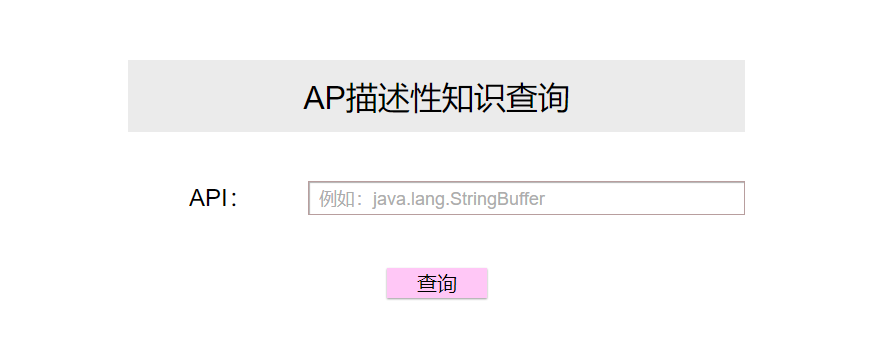
\includegraphics[width=\textwidth]{image/input.png}
    }
    \subfigure[展示界面]{
        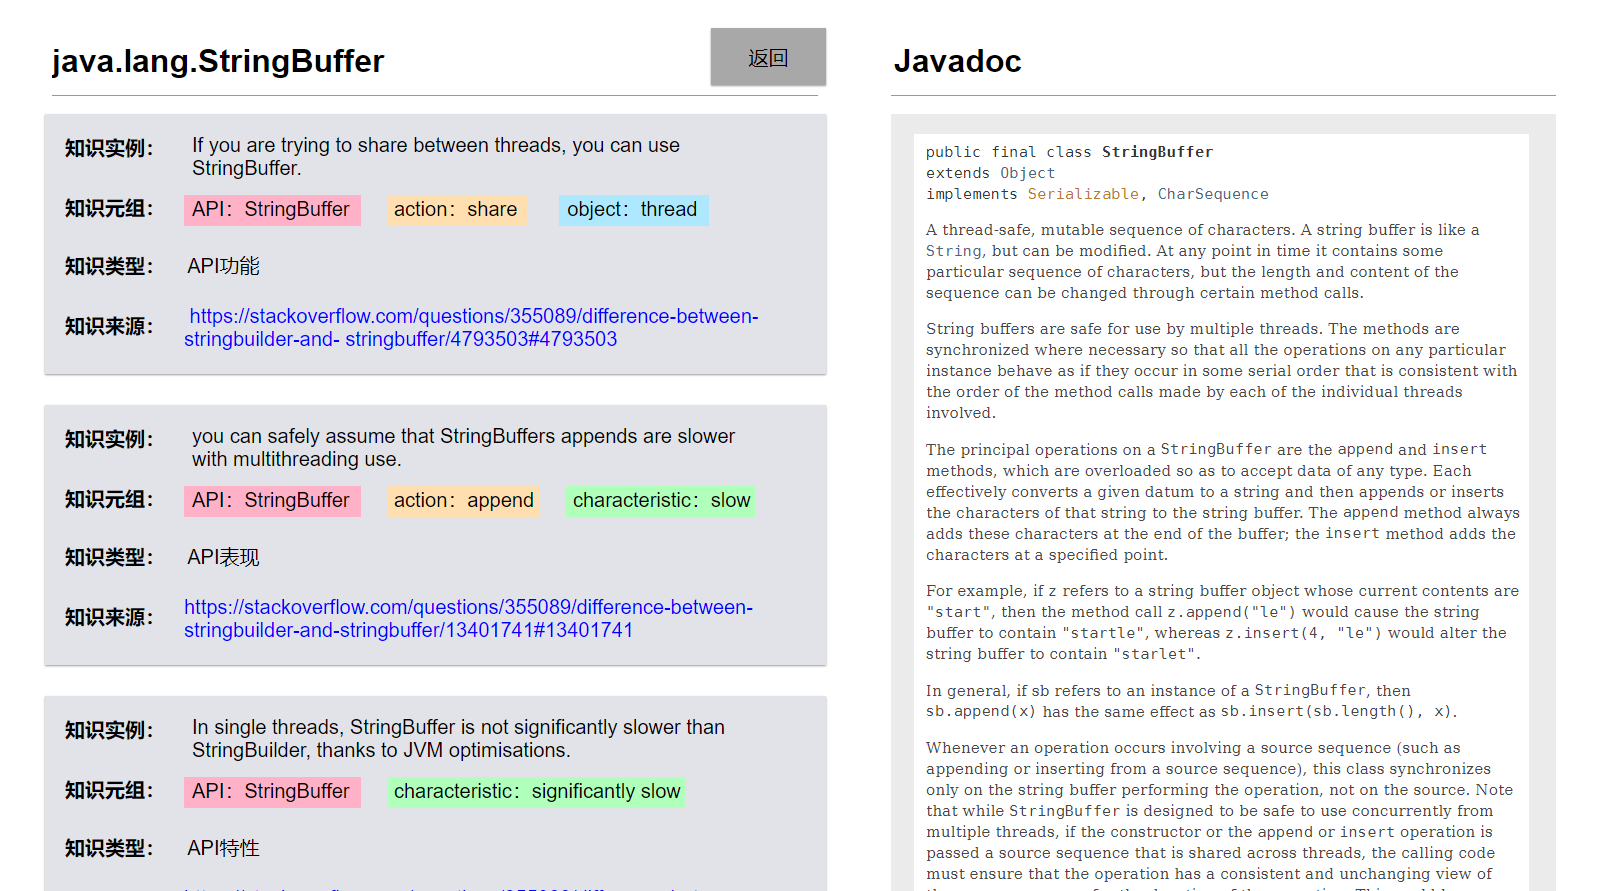
\includegraphics[width=\textwidth]{image/output.png}
    }
    \caption{知识汇总应用前端} 
    \label{fig:fig1} 
\end{figure}

\section{本章小结}
本章介绍了API描述性知识抽取系统及其应用的设计和实现。其中,抽取系统设计为三个模块,分别是语料库生成模块,抽取主体模块以及知识图谱构建模块。本文的应用基于Flask框架、Gunicorn服务器以及Vue框架,实现了一个查询API描述性知识以及相关的API文档的应用。在下一章中,将会对整个系统进行实验评估,以验证本方法的有效性。
